\chapter{Methodology}

\section{Problem Formulation}

This thesis formulates LDCT denoising as a paired supervised image restoration problem. Let \(x \in \mathbb{R}^{H \times W}\) denote a low-dose CT slice and \(y \in \mathbb{R}^{H \times W}\) denote the corresponding normal-dose CT slice. A denoising model \(f_{\theta}\) predicts
\begin{equation}
    \hat{y}=f_{\theta}(x),
\end{equation}
where \(\theta\) represents learnable parameters. The goal is to make \(\hat{y}\) close to \(y\), while preserving anatomical structures in \(x\).

The training objective follows the general supervised restoration setting. The model is optimized on paired LDCT and NDCT patches. Patch-based training is used because full CT slices are memory intensive, especially for Transformer-based restoration models. During evaluation, the model is applied to complete \(512 \times 512\) slices through tiled inference so that final metrics are computed on full images rather than only on training patches.

\section{Dataset and Preprocessing}

The experiments use paired slices prepared from the AAPM-Mayo LDCT dataset \cite{aapm}. The working dataset contains 3mm B30 LDCT and NDCT image pairs from ten patients: L067, L096, L109, L143, L192, L286, L291, L310, L333, and L506. Patient L506 is held out as the test patient. This patient-level split is important because slice-level random splitting can place neighboring slices from the same patient in both training and testing, which may overestimate generalization.

The preprocessing pipeline starts from paired DICOM series. For each patient and dose level, slices are sorted by their axial position, converted from stored pixel values to Hounsfield units (HU) using the DICOM rescale slope and intercept, and saved as paired NumPy arrays. Invalid background values marked as \(-2000\) in the original conversion are set to zero before HU conversion. The HU images are then linearly normalized from \([-1024, 3072]\) to \([0,1]\). No CT display windowing is applied before training; the display window \([-160, 240]\) HU is used only after denormalization for visualization and metric preparation.

Each full slice has spatial size \(512 \times 512\). During training, the data loader samples paired \(64 \times 64\) crops from the same spatial location in the LDCT and NDCT images. The same flip or rotation augmentation is applied to both images in a pair, so the supervised target remains aligned with the low-dose input. The \(64 \times 64\) size is therefore a memory-aware training crop size, not the original image size and not a ViT-style token size. During testing, the model is evaluated on full slices by tiled inference, and the reported metrics are computed on reconstructed \(512 \times 512\) predictions.

\begin{table}[!htbp]
    \centering
    \caption{Dataset split and evaluation protocol.}
    \renewcommand{\arraystretch}{1.35}
    \begin{tabular*}{\textwidth}{>{\raggedright\arraybackslash}p{0.24\textwidth}|>{\raggedright\arraybackslash}p{0.38\textwidth}|>{\raggedright\arraybackslash}p{0.28\textwidth}}
        \hline
        Item & Setting & Purpose \\
        \hline
        Dataset & AAPM-Mayo 3mm B30 paired LDCT/NDCT slices & Supervised low-dose to normal-dose CT restoration \\
        \hline
        Patients & L067, L096, L109, L143, L192, L286, L291, L310, L333, L506 & Patient-level organization of paired slices \\
        \hline
        Test patient & L506 & Held-out evaluation to reduce patient-level leakage \\
        \hline
        Slice count & 2167 training slices and 211 held-out L506 test slices & Explicit patient-level split size \\
        \hline
        Image size & \(512 \times 512\) & Full CT slice denoising and tiled inference \\
        \hline
        Preprocessing & DICOM to HU, paired NumPy saving, normalization from \([-1024,3072]\) to \([0,1]\) & Stable numerical range for supervised training \\
        \hline
        Training samples & Random paired \(64 \times 64\) crops with matched augmentation & Memory-aware training while preserving LDCT/NDCT alignment \\
        \hline
        Metrics & PSNR, SSIM, RMSE, residual correlation, edge leakage & Image quality and residual behavior evaluation \\
        \hline
    \end{tabular*}
    \label{tab:dataset_split}
\end{table}

\section{Baseline Models}

Three types of inputs or models are compared in this thesis. The first is the raw low-dose input, which provides a lower-bound reference. The second is RED-CNN, a CNN-based LDCT denoising model \cite{redcnn}. RED-CNN is used because it is a widely recognized baseline for CT denoising and represents a strong convolutional approach. The third is CTformer, a Transformer-based model designed for LDCT denoising \cite{ctformer}. CTformer is included to compare the proposed CTRestormer with another attention-based CT denoising method.

Using these baselines makes the evaluation more informative. If CTRestormer is compared only with the low-dose input, improvement is expected and not very meaningful. Comparing it with RED-CNN and CTformer shows whether the adapted model is competitive with both CNN and Transformer baselines. This also helps interpret residual behavior: a method with similar PSNR may remove different types of residual signal.

\section{Proposed CTRestormer}

CTRestormer is the Restormer-style model adapted in this thesis for LDCT denoising. It is not presented as a new theory of attention, but as a practical adaptation of high-resolution Transformer restoration to CT images. The model follows the idea that image restoration should preserve spatial detail while learning the degradation-specific correction. Compared with classification-oriented Transformers, restoration Transformers must output dense images and maintain local alignment.

\begin{figure}[!htbp]
    \centering
    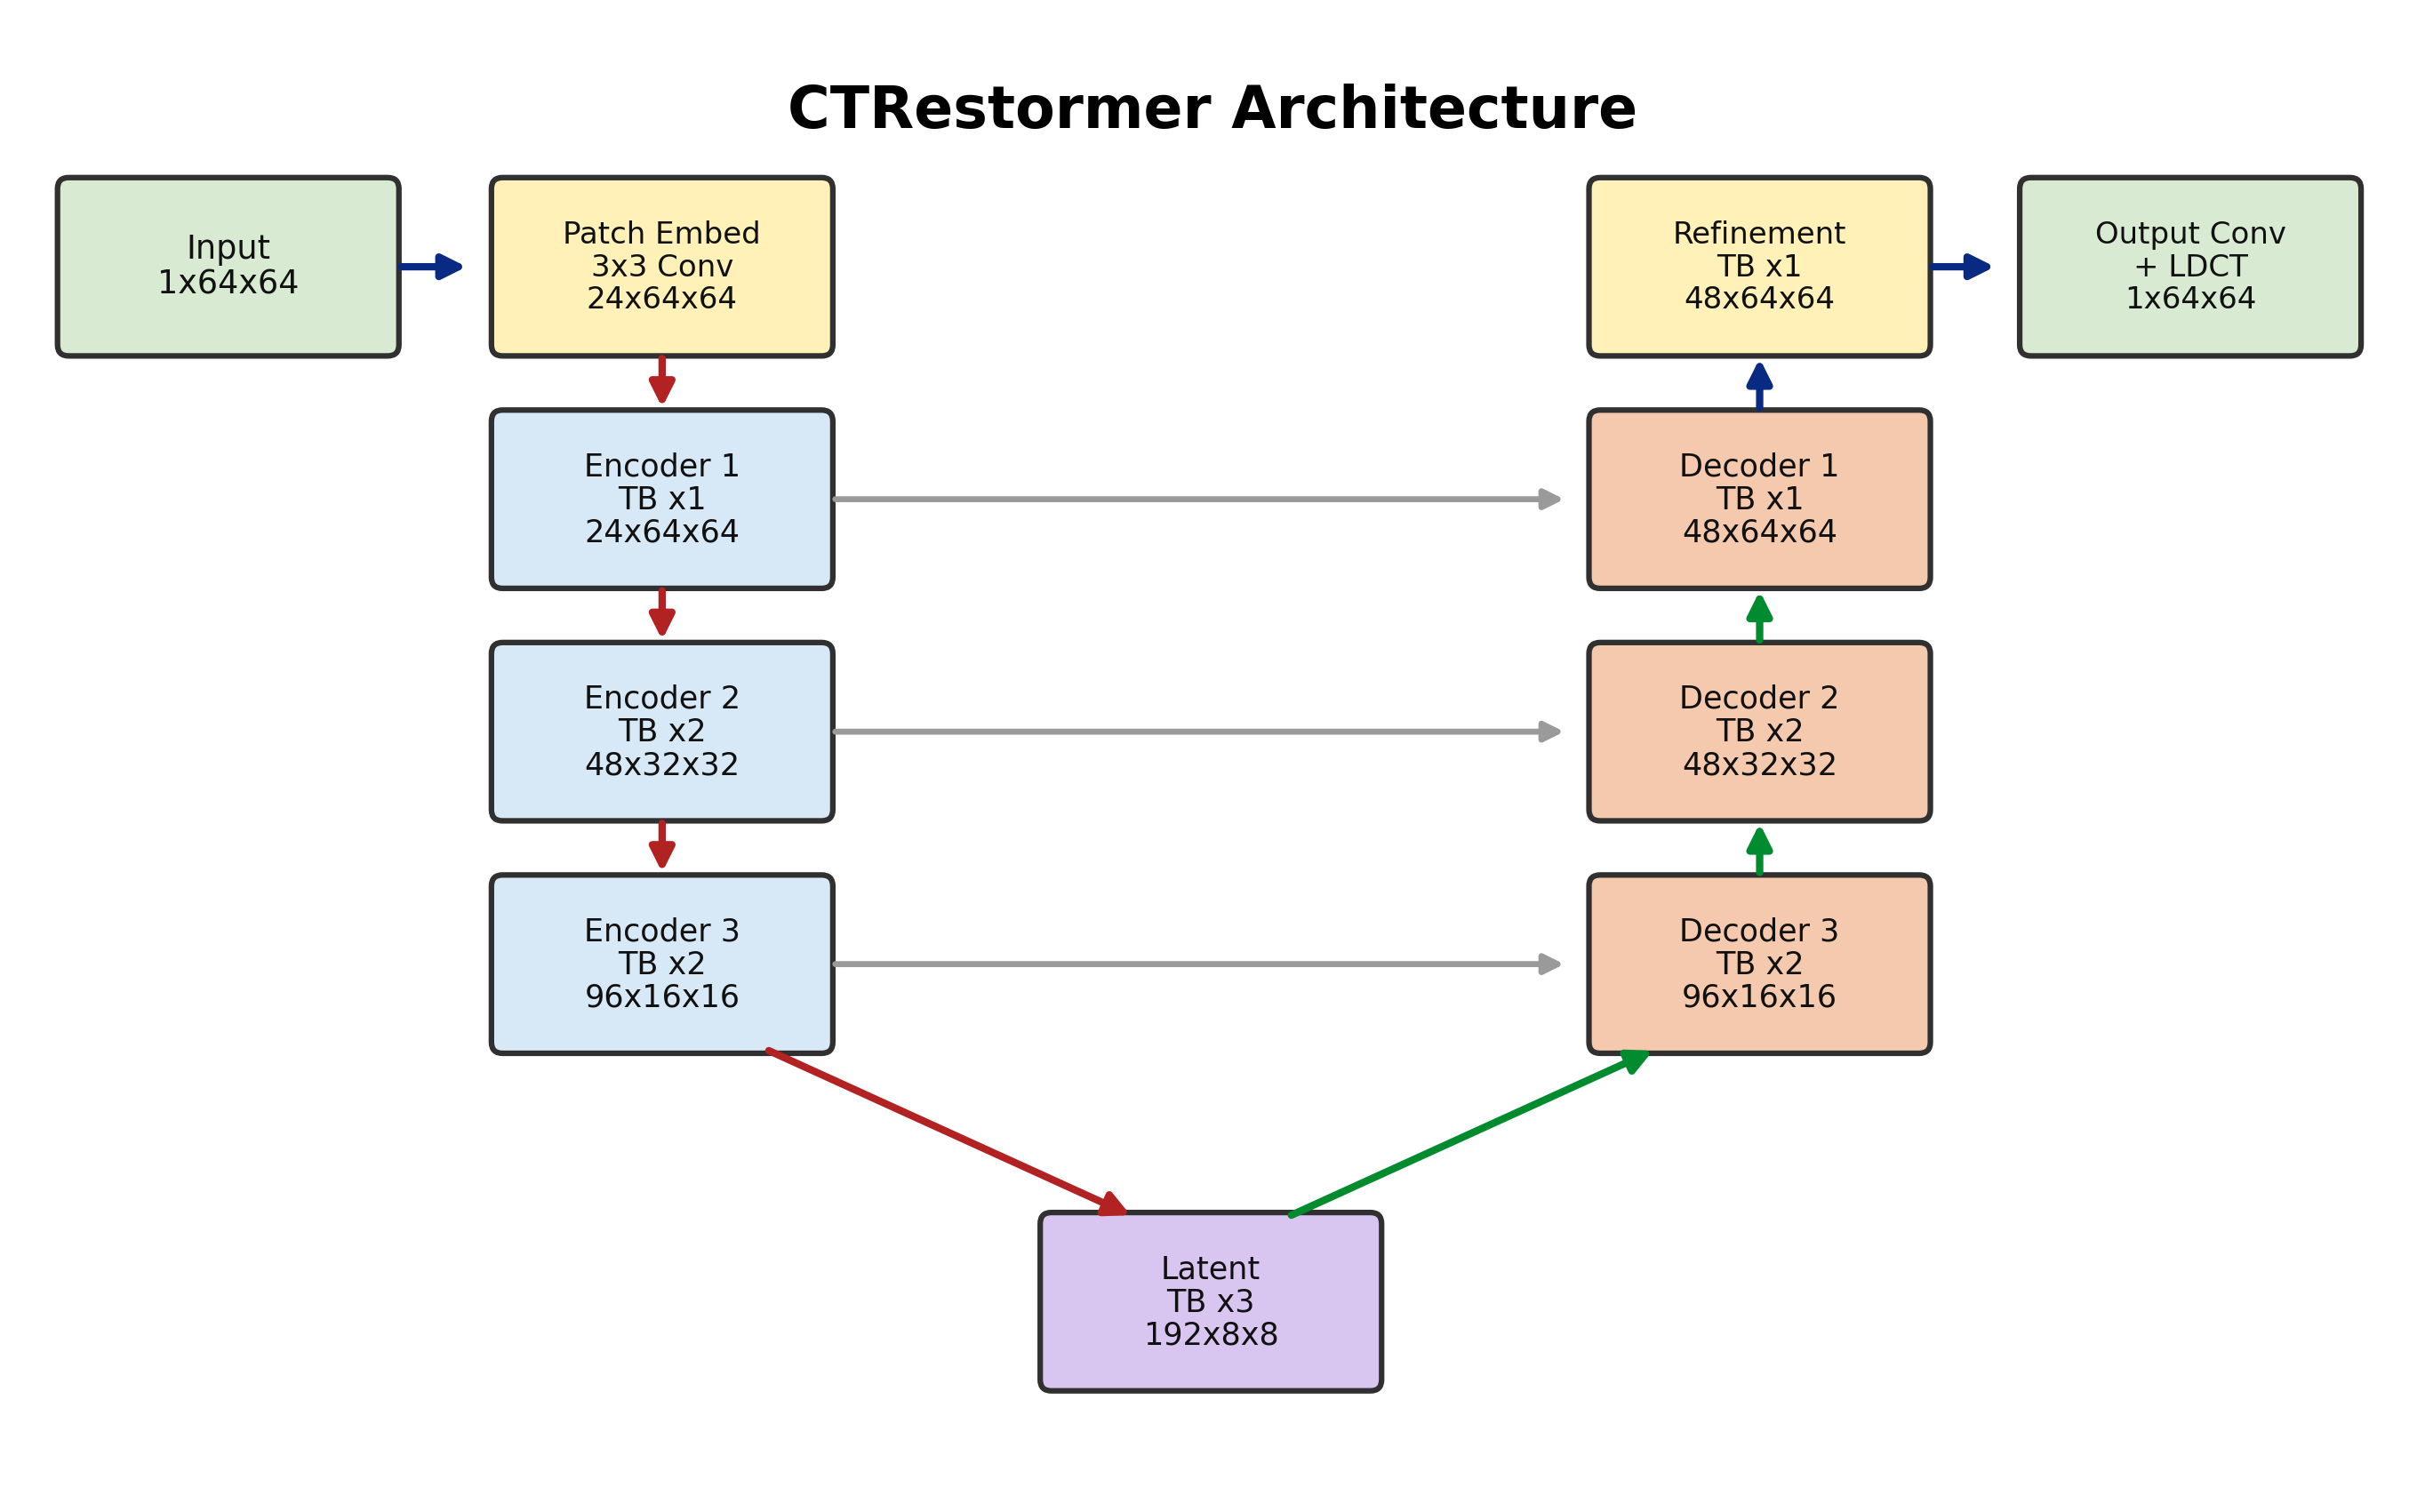
\includegraphics[width=0.98\textwidth]{images/ctrestormer_architecture.png}
    \caption{Compact CTRestormer architecture used in this thesis. Red arrows indicate downsampling, green arrows indicate upsampling, and gray arrows indicate encoder-decoder skip connections. The highlighted dimensions show the feature size at each stage.}
    \label{fig:ctrestormer_arch}
\end{figure}

The proposed pipeline uses overlap patch embedding, hierarchical feature processing, Transformer restoration blocks, skip-connected decoding, refinement blocks, and residual output prediction, as shown in Figure \ref{fig:ctrestormer_arch}. The actual trained configuration uses base dimension 24. For a \(64 \times 64\) training crop, the model input tensor is \(1 \times 64 \times 64\). The first model layer is an overlap patch embedding layer implemented as a \(3 \times 3\) convolution with stride 1 and padding 1. It maps the input to a \(24 \times 64 \times 64\) feature map while keeping the spatial resolution unchanged.

This step should not be confused with ViT-style patch tokenization. In ViT, an image is commonly divided into non-overlapping patches and converted into a token sequence before Transformer processing. In the CTRestormer implementation used here, the \(64 \times 64\) crop remains a two-dimensional feature map. The patch embedding is a convolutional feature projection, not a preprocessing step outside the network. The feature map then passes through three downsampling stages to \(48 \times 32 \times 32\), \(96 \times 16 \times 16\), and \(192 \times 8 \times 8\). The decoder reconstructs high-resolution features with PixelShuffle upsampling, skip fusion, and channel reduction. After the final skip concatenation, the high-resolution decoder and refinement stages operate on \(48 \times 64 \times 64\) features. The final output convolution predicts a residual correction that is added to the LDCT input.

Each Transformer restoration block (TB) contains two residual sub-blocks, as shown in Figure \ref{fig:tb_block}. The first sub-block applies two-dimensional layer normalization followed by an MDTA-style attention module. In this implementation, query, key, and value features are generated by \(1 \times 1\) convolution and depthwise \(3 \times 3\) convolution, so the attention branch still contains local spatial mixing. The second sub-block applies another normalization and a gated depthwise feed-forward network (GDFN). A TB keeps the spatial size unchanged; only the channel count \(C\) depends on the current encoder or decoder level. This combination is useful for image restoration because it combines attention-based feature interaction with convolution-like local bias.

\begin{figure}[!htbp]
    \centering
    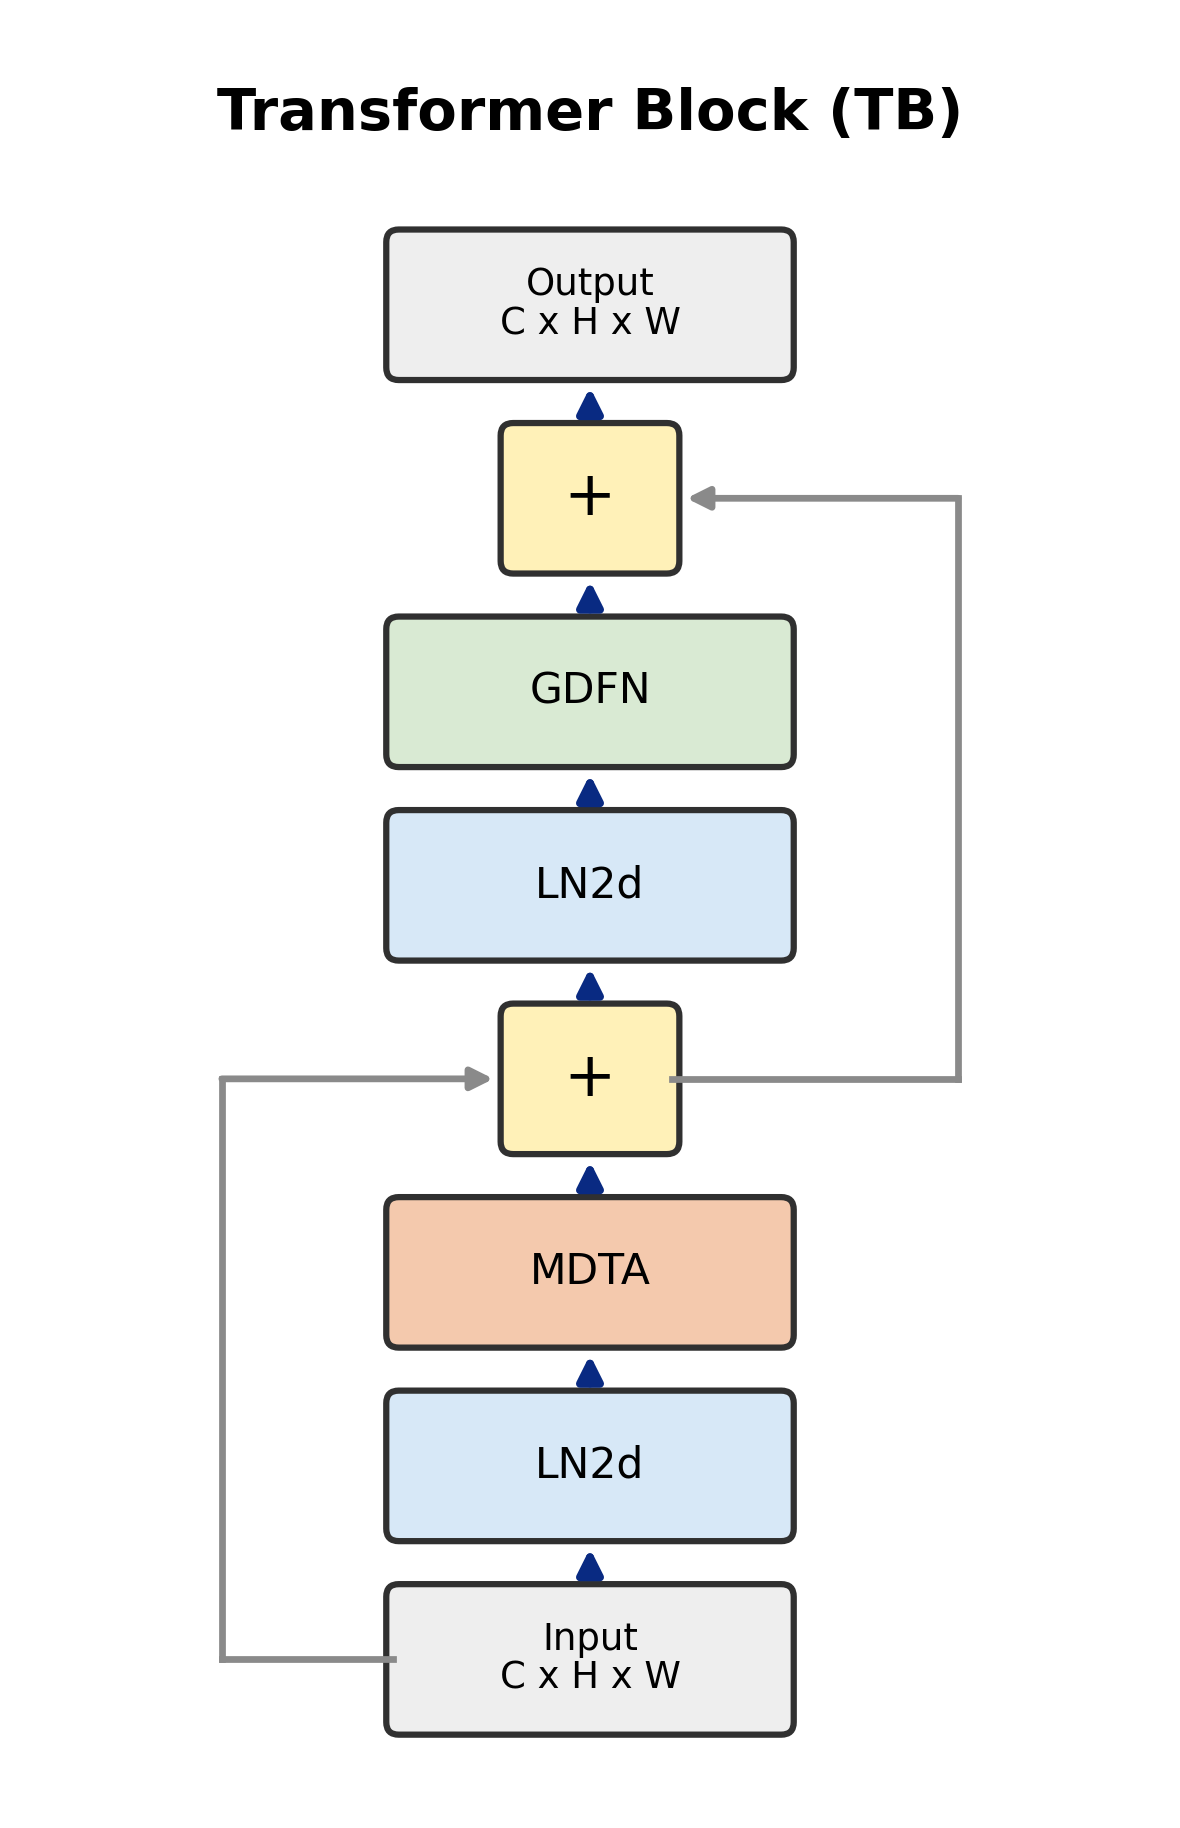
\includegraphics[width=0.45\textwidth]{images/ctrestormer_tb_block.png}
    \caption{Transformer restoration block used in CTRestormer. Each TB keeps the input feature size \(C \times H \times W\), applies an attention residual branch and a gated feed-forward residual branch, and preserves spatial alignment for dense image restoration.}
    \label{fig:tb_block}
\end{figure}

In Figure \ref{fig:tb_block}, LN2d denotes two-dimensional layer normalization applied on feature maps. Unlike the layer normalization used for one-dimensional token sequences, LN2d normalizes the channel features while preserving the \(H \times W\) spatial layout. MDTA denotes the attention branch, where query, key, and value features are produced by convolutional projections. GDFN denotes the gated depthwise feed-forward network, which expands channels, applies depthwise spatial mixing, and uses a gated nonlinearity before projecting features back. The \(+\) symbols denote residual addition: the block adds the branch output back to its input feature map. These residual connections help stabilize training and preserve anatomical information by allowing the model to learn feature corrections rather than replacing the whole representation.

The architecture is effective for LDCT denoising for several reasons. First, overlap patch embedding avoids hard patch boundaries and preserves local continuity in CT images. Second, the encoder-decoder hierarchy lets the model combine fine local texture with larger contextual information. Third, skip connections pass high-resolution structure from the encoder to the decoder, which helps preserve anatomical boundaries. Fourth, residual output prediction constrains the model to learn a correction between LDCT and NDCT instead of generating a completely new image. Finally, tiled inference makes the model practical for full \(512 \times 512\) CT slices even though full-image attention would exceed memory limits.

Compared with RED-CNN, CTRestormer has stronger long-range feature interaction. RED-CNN is stable and efficient, but its convolutional layers mainly aggregate local neighborhoods and do not explicitly model global dependencies. This can limit its ability to distinguish structured artifacts from anatomical texture. Compared with the local CTformer implementation, CTRestormer has a more restoration-oriented hierarchy. CTformer uses token-to-token encoding and a shallow Transformer bottleneck in this project, which is lightweight but less expressive for multi-scale image restoration. CTRestormer adds a U-shaped reconstruction path, explicit skip fusion, deeper restoration blocks, and residual prediction; these choices make it more suitable for dense denoising.

\begin{figure}[!htbp]
    \centering
    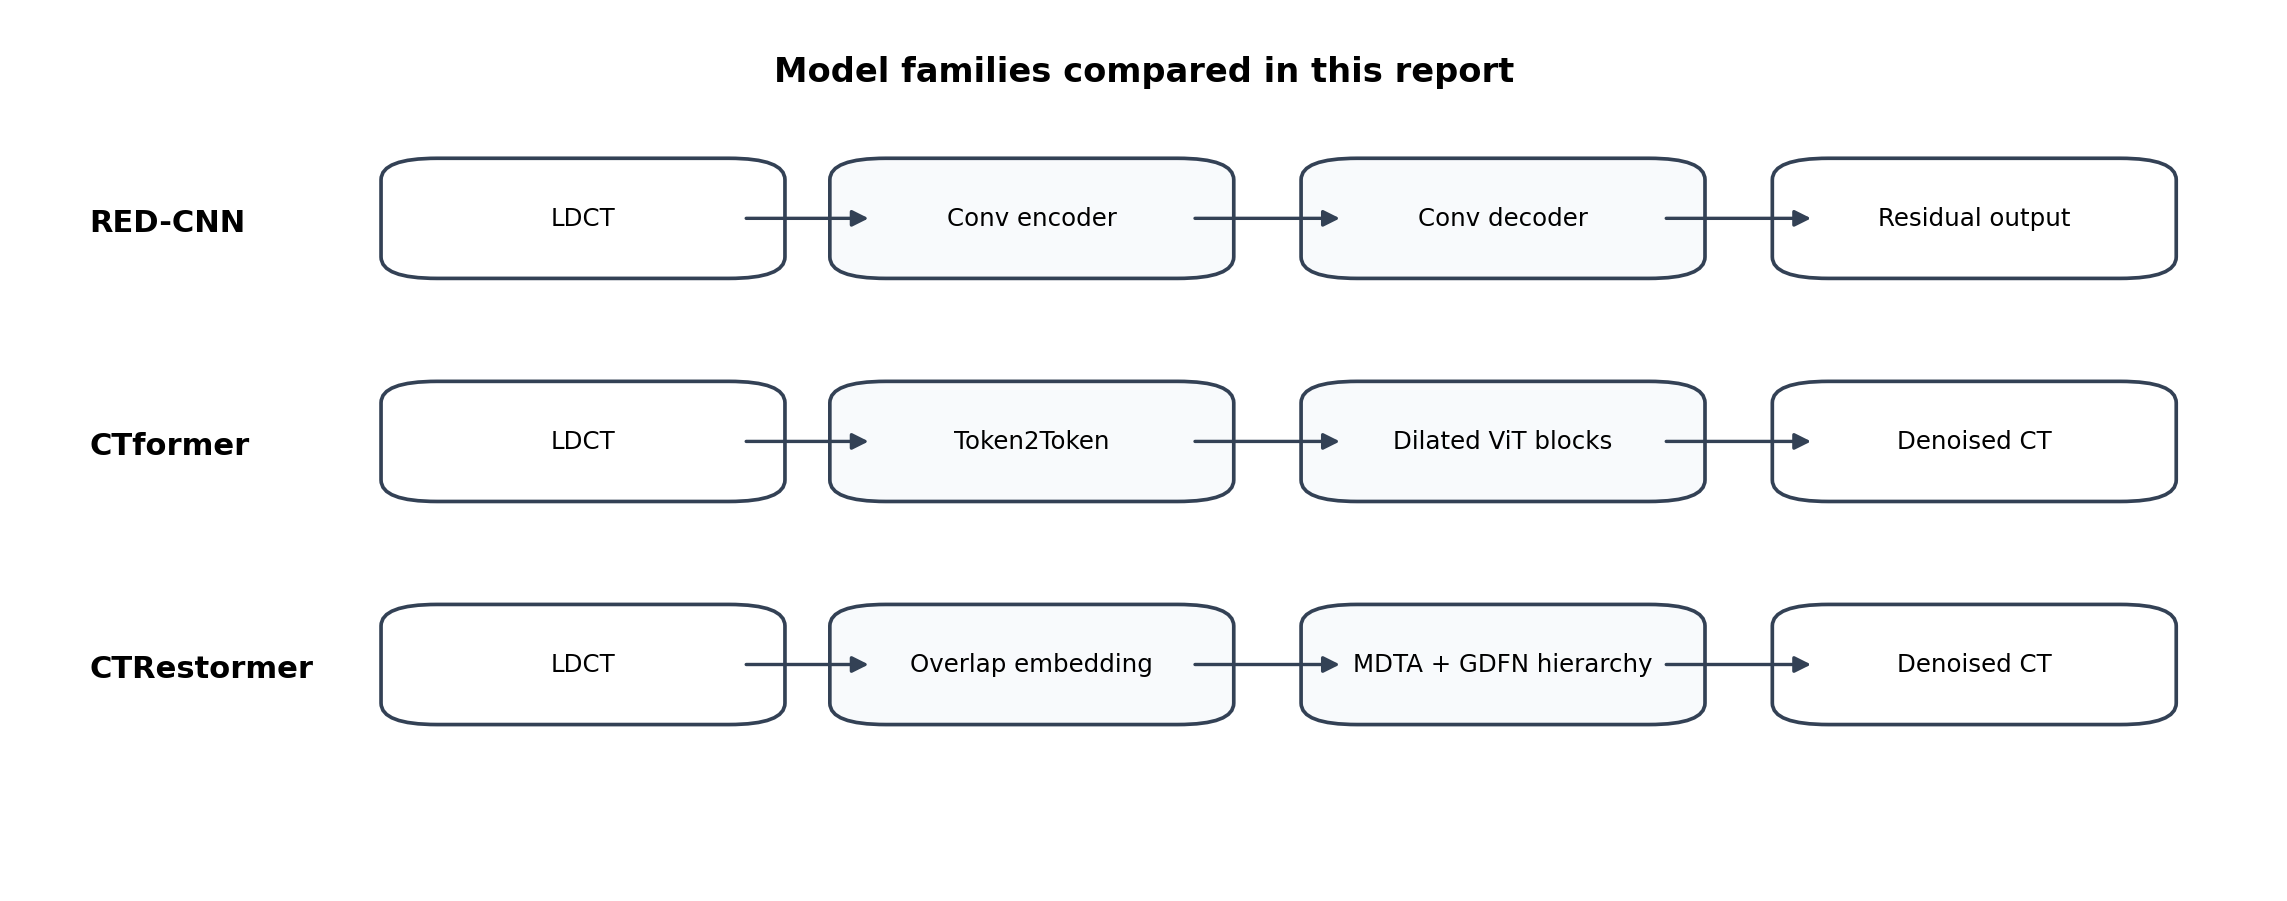
\includegraphics[width=0.82\textwidth]{images/model_comparison_schematic.png}
    \caption{Schematic comparison of the evaluated denoising models. RED-CNN represents a convolutional baseline, CTformer represents a CT-specific Transformer baseline, and CTRestormer is the Restormer-style model adapted in this thesis.}
    \label{fig:model_schematic}
\end{figure}

\section{Memory-Aware Training and Tiled Inference}

High-resolution Transformer restoration can be limited by GPU memory. A full \(512 \times 512\) CT slice contains many spatial tokens, and attention-based modules can be expensive. Therefore, the implementation uses memory-aware training and inference strategies. During training, patches are sampled from paired slices. Patch-based training reduces memory usage and increases the number of local training samples. Mixed precision and gradient accumulation can further improve practical feasibility on limited hardware.

During inference, tiled prediction is used to reconstruct full slices. In the current implementation, a \(512 \times 512\) slice is padded and divided into overlapping \(64 \times 64\) tiles with stride 32. Each tile is processed by the model, and the central regions of the tile predictions are aggregated into a full \(512 \times 512\) output. Tiled inference avoids out-of-memory errors while still allowing metrics to be computed on complete slices. This engineering detail is important because the goal of LDCT denoising is full-image restoration, not only patch-level prediction.

\section{Residual Noise Analysis}

To analyze what each model removes, this thesis defines three residual quantities:
\begin{equation}
    r_{\mathrm{true}} = x-y,
\end{equation}
\begin{equation}
    r_{\mathrm{removed}} = x-\hat{y},
\end{equation}
\begin{equation}
    e_{\mathrm{pred}} = \hat{y}-y.
\end{equation}
Here \(r_{\mathrm{true}}\) is the estimated LDCT residual relative to the NDCT target, \(r_{\mathrm{removed}}\) is the residual removed by the model, and \(e_{\mathrm{pred}}\) is the remaining prediction error. If a model removes noise in a desirable way, \(r_{\mathrm{removed}}\) should share texture and distributional similarity with \(r_{\mathrm{true}}\), while containing limited anatomical edge information.

The first residual metric is residual correlation:
\begin{equation}
    \rho = \mathrm{corr}(r_{\mathrm{true}}, r_{\mathrm{removed}}).
\end{equation}
A higher correlation suggests that the removed residual is more aligned with the estimated LDCT noise, although this metric alone is not sufficient to prove clinical safety. The second metric is the standard deviation of the removed residual, which measures removal strength. The third metric is edge leakage. It estimates how strongly the removed residual overlaps with edge-like structures. Higher edge leakage indicates a stronger risk that the model removes anatomical boundary information together with noise.

\begin{figure}[!htbp]
    \centering
    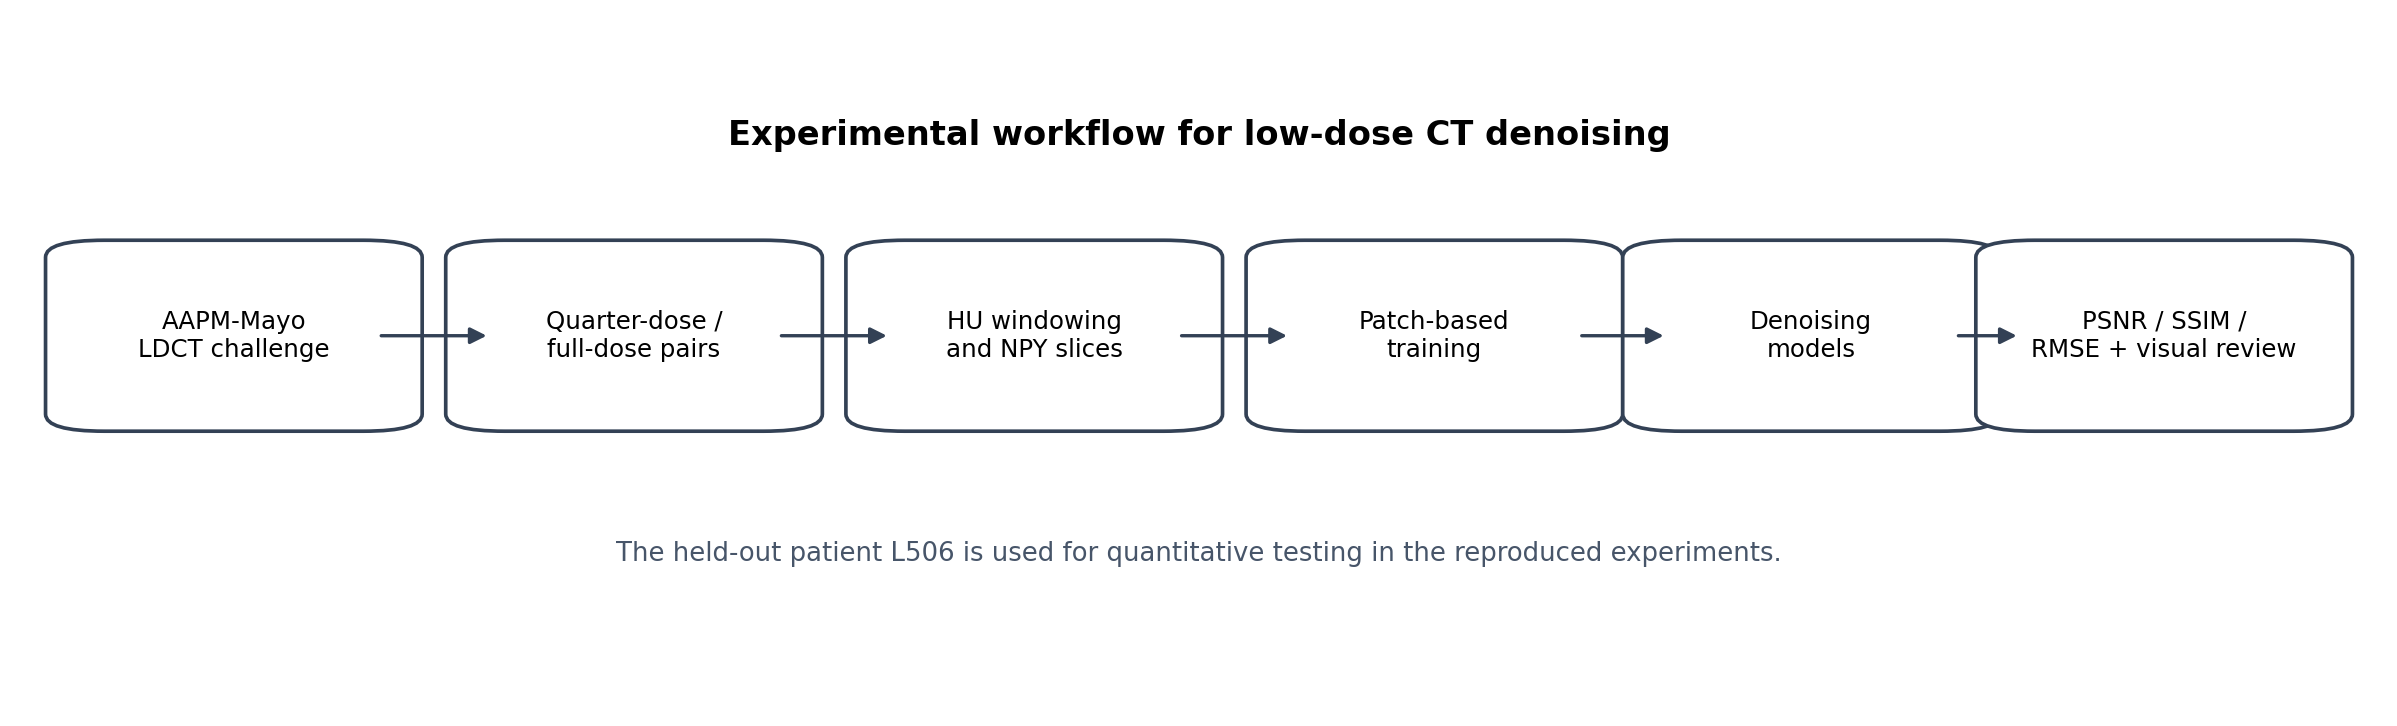
\includegraphics[width=0.82\textwidth]{images/experimental_workflow.png}
    \caption{Experimental workflow from paired LDCT/NDCT preparation to model training, full-slice inference, metric evaluation, and residual analysis.}
    \label{fig:workflow}
\end{figure}
